\section{Bloque 1. Computacion reversible y oráculos booleanos}\label{sec:bloque_1}
\subsection{Ejercicio 1.1. Puerta AND reversible}
Se implementa $|a_1a_0\rangle|0\rangle \to |a_1a_0\rangle|a_1\wedge a_0\rangle$ con una puerta Toffoli: controles
en $q_0\equiv a_0$ y $q_1\equiv a_1$, objetivo en la ancilla $q_2\equiv y$, inicializada a $|0\rangle$.
Cada entrada clásica se prepara con puertas $X$ y se miden los tres qubits; la cadena medida es \texttt{y a1 a0} ($c_2c_1c_0$).

\textbf{Predicción.} La tabla de verdad del AND con las entradas intactas. Como el circuito es determinista,
cada entrada debe dar un único resultado con probabilidad 1.

La puerta Toffoli se muestra en la Figura~\ref{fig:bloque1_e1_1_andtoffoli}.
\begin{figure}[h]
    \centering
    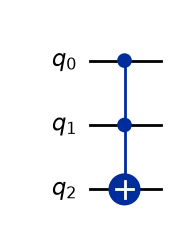
\includegraphics[width=0.15\textwidth]{imagenes/bloque1/e1_1_andtoffoli.png}
    \caption{Puerta Toffoli.}\label{fig:bloque1_e1_1_andtoffoli}
\end{figure}

\begin{figure}[htbp]
    \centering
    \begin{subfigure}{0.4\textwidth}
        \centering
        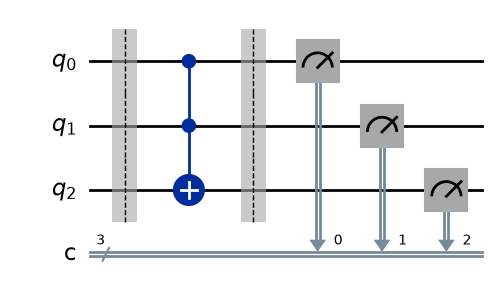
\includegraphics[width=\textwidth]{imagenes/bloque1/e1_1_caso00.png}
        \caption{}
    \end{subfigure}
    \hfill
    \begin{subfigure}{0.4\textwidth}
        \centering
        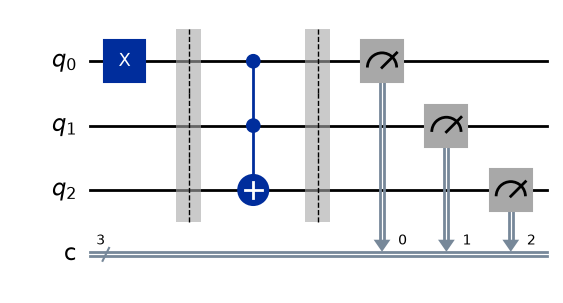
\includegraphics[width=\textwidth]{imagenes/bloque1/e1_1_caso01.png}
        \caption{}
    \end{subfigure}
    \hfill
    \begin{subfigure}{0.4\textwidth}
        \centering
        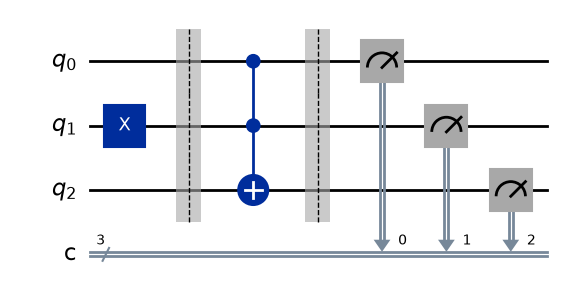
\includegraphics[width=\textwidth]{imagenes/bloque1/e1_1_caso10.png}
        \caption{}
    \end{subfigure}
    \hfill
    \begin{subfigure}{0.4\textwidth}
        \centering
        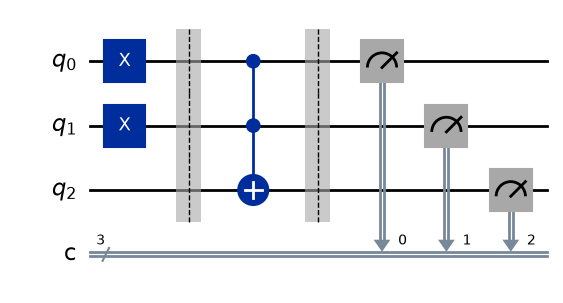
\includegraphics[width=\textwidth]{imagenes/bloque1/e1_1_caso11.png}
        \caption{}
    \end{subfigure}
    \caption{Circuitos de puerta $AND$ para entradas $q_1, q_0 = 00, 01, 10, 11$.}\label{fig:bloque1_e1_1_circuitos}
\end{figure}

La Tabla~\ref{tab:bloque1_e1_1} recoge la tabla de verdad simulada junto a la teórica.

\begin{table}[htbp]
    \centering
\begin{tabular}{c|c|c|c|c}
\hline
$a_1a_0$ & $f(x)$ teórica & $f(x)$ simulada & $x$ tras $U_f$ & Prob. \\
\hline
\texttt{00} & \texttt{0} & \texttt{0} & \texttt{00} & 1 \\
\texttt{01} & \texttt{0} & \texttt{0} & \texttt{01} & 1 \\
\texttt{10} & \texttt{0} & \texttt{0} & \texttt{10} & 1 \\
\texttt{11} & \texttt{1} & \texttt{1} & \texttt{11} & 1 \\
\hline
\end{tabular}
    \caption{Ejercicio 1.1: tabla de verdad del AND reversible. La columna $x$ tras $U_f$ es la entrada medida después del oráculo.}\label{tab:bloque1_e1_1}
\end{table}

\textbf{Resultado.} Para las cuatro entradas la salida medida coincide con la tabla de verdad del AND ($y=1$ únicamente para $a_1a_0=11$),
con probabilidad 1 y sin ningún otro resultado. Los qubits de entrada se miden exactamente en el estado en que se prepararon: el oráculo conserva la entrada
y escribe $f(a)$ en la ancilla mediante una suma módulo 2, y eso es lo que hace reversible un AND (que por sí solo no lo es, ya que a partir de la salida no se pueden
recuperar las entradas). La matriz del circuito coincide con la permutación $|x\rangle|y\rangle\mapsto|x\rangle|y\oplus f(x)\rangle$ y cumple $U_f^2=I$.

%--------------------------------------------------------------------
\subsection{Ejercicio 1.2. Paralelismo cuántico}

Se aplican puertas $H$ a $q_0$ y $q_1$ para preparar $\tfrac12(|00\rangle+|01\rangle+|10\rangle+|11\rangle)|0\rangle$ y después el oráculo. Por linealidad:

$$U_f\Big(\tfrac12\sum_{a_1a_0}|a_1a_0\rangle\Big)|0\rangle=\tfrac12\big(|00\rangle|0\rangle+|01\rangle|0\rangle+|10\rangle|0\rangle+|11\rangle|1\rangle\big).$$

En la Figura~\ref{fig:bloque1_e1_2_circuito} se muestra el circuito correspondiente.

\begin{figure}[h]
     \centering
    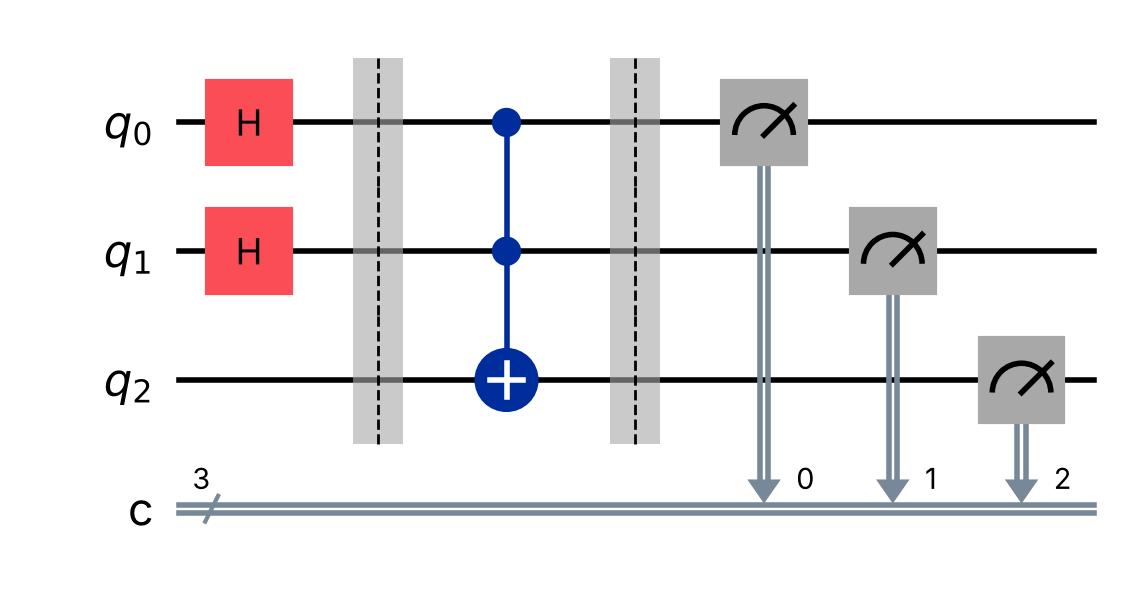
\includegraphics[width=0.5\textwidth]{imagenes/bloque1/e1_2_circuito.png}
    \caption{Circuito completo.}\label{fig:bloque1_e1_2_circuito}
\end{figure}

\textbf{Predicción.} Al medir los tres qubits aparecen cuatro cadenas \texttt{y a1 a0}: \texttt{000}, \texttt{001}, \texttt{010} y \texttt{111},
cada una con probabilidad $1/4$. Se obtiene el estado teórico con \texttt{Statevector} (circuito sin medidas) y se compara con el histograma simulado con \texttt{AerSimulator}
mediante un test $\chi^2$ de bondad de ajuste.

\begin{figure}[htbp]
    \centering
    \begin{subfigure}{0.48\textwidth}
        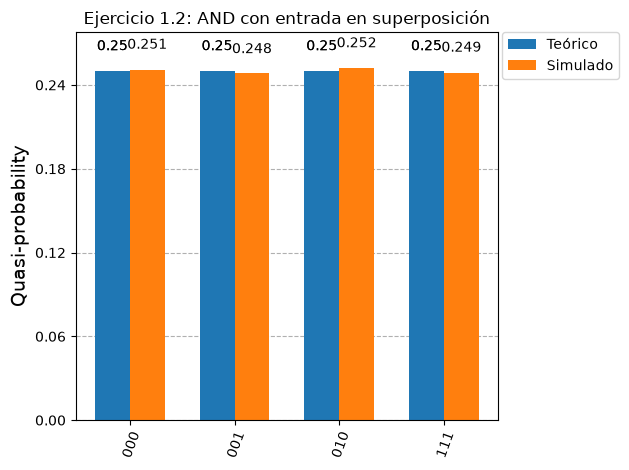
\includegraphics[width=0.9\textwidth]{imagenes/bloque1/e1_2_comp_prediccionTeoria.png}
        \caption{}
    \end{subfigure}
    \hfill
    \begin{subfigure}{0.48\textwidth}
        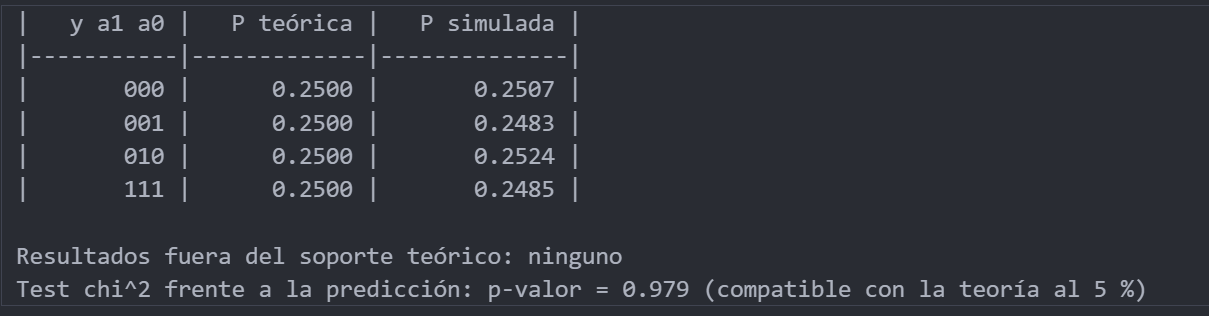
\includegraphics[width=0.9\textwidth]{imagenes/bloque1/e1_2_tabla_comparacion.png}
        \caption{}
    \end{subfigure}
    \caption{(a): Comparación de los histogramas de la predicción teórica y de la simulación.\\
    (b): Tabla comparativa de las probabilidades teóricas y de simulación, con ajuste positivo de $\chi^2$.}\label{fig:bloque1_e1_2_comparacion}
\end{figure}

En la Figura~\ref{fig:bloque1_e1_2_comparacion} se observa que las probabilidades obtenidas en la simulación son prácticamente idénticas a las
teóricas, con pequeñas desviaciones. En el test $\chi^2$ de bondad de ajuste frente a la predicción teórica se obtiene un $p$-valor de $0{,}979$,
compatible con la teoría al $5\%$: las discrepancias entre los datos observados y los predichos son muy pequeñas y
encajan con las fluctuaciones estadísticas esperables con 4096 disparos.

\textbf{¿Y con un solo disparo?} Para comprobarlo experimentalmente se ejecuta el circuito con \emph{un único disparo} en diez ocasiones
independientes (cambiando la semilla del simulador en cada una) y se anota la fila \texttt{y a1 a0} obtenida. En todas las ejecuciones se
obtiene una única fila, distinta de una ejecución a otra, y tras las diez ejecuciones se han visto tres de las cuatro filas posibles: ninguna ejecución
individual da la tabla completa. Después se almacena el resultado de cada disparo de una misma tanda y se cuenta cuántas filas distintas se han observado
tras $k$ disparos (Figura~\ref{fig:bloque1_e1_2_experimento}, izquierda): en la tanda de 40 disparos la tabla se completa en el disparo número 5, no antes.

\begin{figure}[htbp]
    \centering
    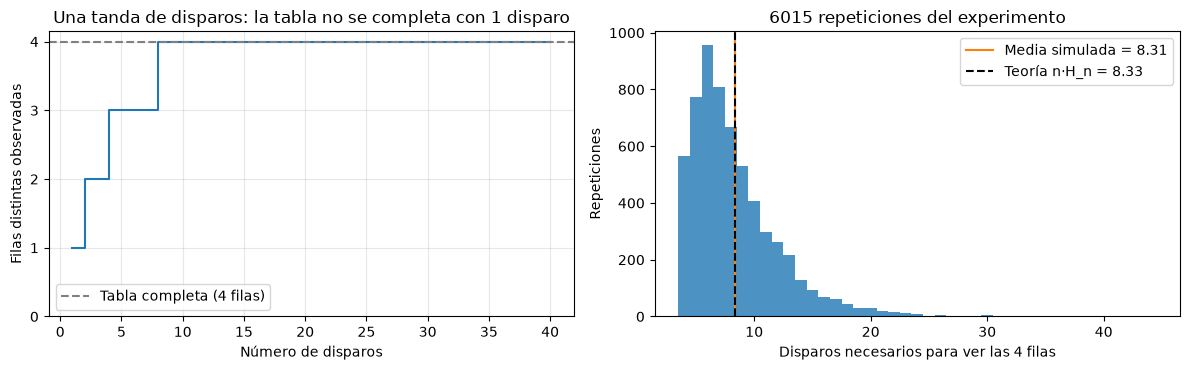
\includegraphics[width=\textwidth]{imagenes/bloque1/e1_2_experimento_1_disparo.png}
    \caption{Experimento de un solo disparo en el ejercicio 1.2.
    Izquierda: filas distintas observadas en función del número de disparos en una tanda; la curva parte de una sola fila y necesita varios disparos para llegar a las cuatro.
    Derecha: histograma del número de disparos necesarios para observar las cuatro filas, repitiendo el experimento 6034 veces; la media simulada ($8{,}29$)
    coincide con la teórica $nH_n=25/3\approx 8{,}33$.}\label{fig:bloque1_e1_2_experimento}
\end{figure}

El histograma de la derecha de la Figura~\ref{fig:bloque1_e1_2_experimento} muestra que el mínimo número de disparos necesarios es 4 y que la distribución tiene una cola larga hacia la derecha
(en algunas repeticiones se necesitan más de 20 disparos). Incluso con exactamente 4 disparos solo se obtiene la tabla completa con probabilidad
$4!/4^4=24/256\approx 9{,}4\%$ (en la simulación, un $9{,}8\%$), mientras que con un solo disparo esa probabilidad es exactamente 0.

%--------------------------------------------------------------------
\subsection{Ejercicio 1.3. Puerta XOR reversible}
Se repiten los ejercicios 1.1 y 1.2 para $f(a_1,a_0)=a_1\oplus a_0$, que se implementa con dos CNOT que comparten objetivo (la ancilla $q_2$):
\texttt{cx(0,2)} y \texttt{cx(1,2)}. El oráculo se muestra en la Figura~\ref{fig:bloque1_e1_3_xor}.

\begin{figure}[h]
    \centering
    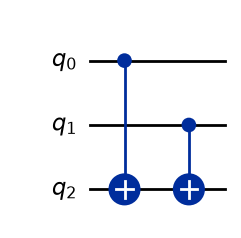
\includegraphics[width=0.3\textwidth]{imagenes/bloque1/e1_3_xor.png}
    \caption{Oráculo XOR reversible con dos puertas CNOT.}\label{fig:bloque1_e1_3_xor}
\end{figure}

\textbf{Predicción con entradas clásicas.} La tabla de verdad del XOR, con las entradas intactas y un único resultado con probabilidad 1 para cada una.

\textbf{Predicción con entrada en superposición.}
$$U_f\Big(\tfrac12\sum_{a_1a_0}|a_1a_0\rangle\Big)|0\rangle=\tfrac12\big(|00\rangle|0\rangle+|01\rangle|1\rangle+|10\rangle|1\rangle+|11\rangle|0\rangle\big),$$
es decir, las cadenas \texttt{y a1 a0} = \texttt{000}, \texttt{101}, \texttt{110} y \texttt{011}, cada una con probabilidad $1/4$.

\begin{figure}[htbp]
    \centering
    \begin{subfigure}{0.4\textwidth}
        \centering
        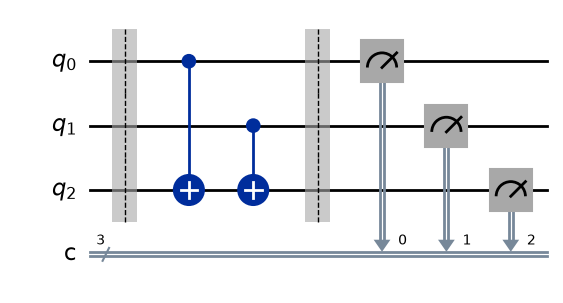
\includegraphics[width=\textwidth]{imagenes/bloque1/e1_3_circuito00.png}
        \caption{}
    \end{subfigure}
    \hfill
    \begin{subfigure}{0.4\textwidth}
        \centering
        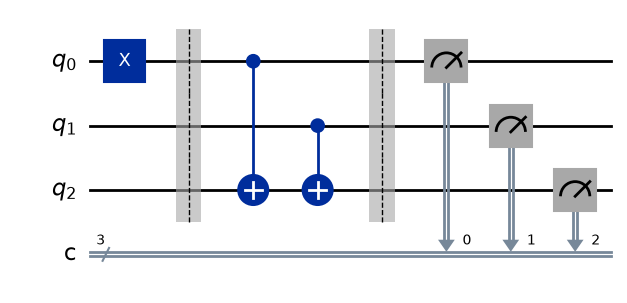
\includegraphics[width=\textwidth]{imagenes/bloque1/e1_3_circuito01.png}
        \caption{}
    \end{subfigure}
    \hfill
    \begin{subfigure}{0.4\textwidth}
        \centering
        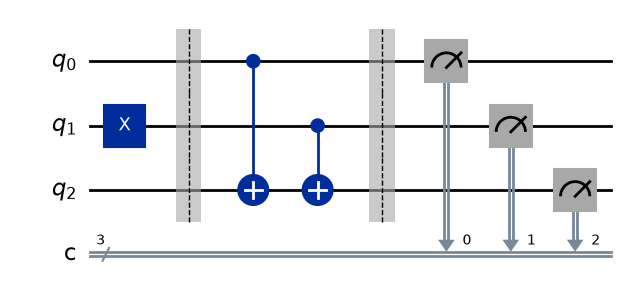
\includegraphics[width=\textwidth]{imagenes/bloque1/e1_3_circuito10.png}
        \caption{}
    \end{subfigure}
    \hfill
    \begin{subfigure}{0.4\textwidth}
        \centering
        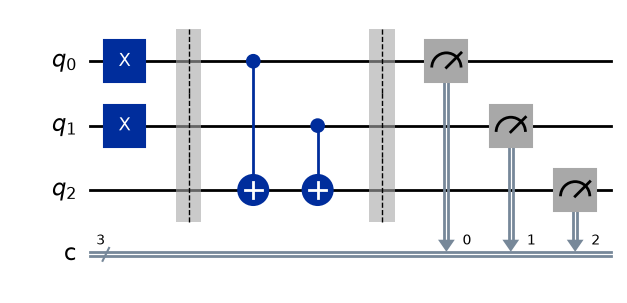
\includegraphics[width=\textwidth]{imagenes/bloque1/e1_3_circuito11.png}
        \caption{}
    \end{subfigure}
    \caption{Circuitos de puerta $XOR$ para entradas $q_1, q_0 = 00, 01, 10, 11$.}\label{fig:bloque1_e1_3_circuitos}
\end{figure}

\begin{table}[htbp]
    \centering
\begin{tabular}{c|c|c|c|c}
\hline
$a_1a_0$ & $f(x)$ teórica & $f(x)$ simulada & $x$ tras $U_f$ & Prob. \\
\hline
\texttt{00} & \texttt{0} & \texttt{0} & \texttt{00} & 1 \\
\texttt{01} & \texttt{1} & \texttt{1} & \texttt{01} & 1 \\
\texttt{10} & \texttt{1} & \texttt{1} & \texttt{10} & 1 \\
\texttt{11} & \texttt{0} & \texttt{0} & \texttt{11} & 1 \\
\hline
\end{tabular}
    \caption{Ejercicio 1.3: tabla de verdad del XOR reversible.}\label{tab:bloque1_e1_3}
\end{table}

La Tabla~\ref{tab:bloque1_e1_3} muestra que, para las cuatro entradas clásicas, la salida simulada coincide con la tabla de verdad del XOR con probabilidad 1 y que
la entrada no se modifica. Con la entrada en superposición se utiliza el circuito de la Figura~\ref{fig:bloque1_e1_3_super} y se compara la distribución
medida con la predicha (Figura~\ref{fig:bloque1_e1_3_comparacion}).

\begin{figure}[h]
    \centering
    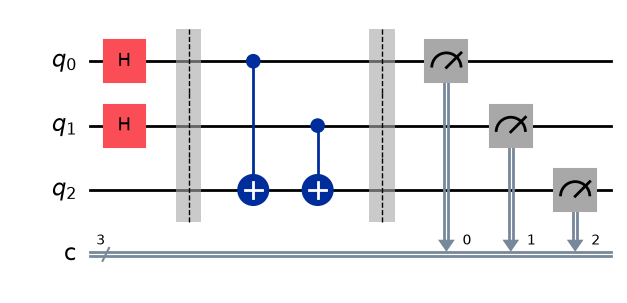
\includegraphics[width=0.5\textwidth]{imagenes/bloque1/e1_3_circuitoXOR_super.png}
    \caption{Circuito XOR con las entradas en superposición.}\label{fig:bloque1_e1_3_super}
\end{figure}

\begin{figure}[h]
    \centering
    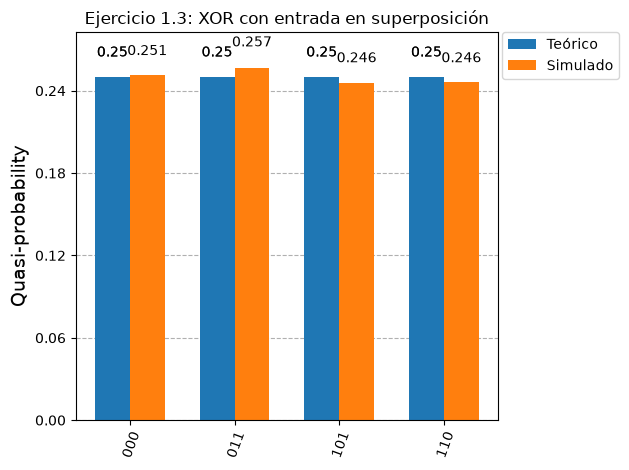
\includegraphics[width=0.6\textwidth]{imagenes/bloque1/e1_3_prediccion_teoria.png}
    \caption{Ejercicio 1.3: comparación entre la predicción teórica y la simulación con la entrada en superposición.}\label{fig:bloque1_e1_3_comparacion}
\end{figure}

\begin{table}[h]
    \centering
    \begin{tabular}{c|c|c}
    \hline
    \texttt{y a1 a0} & $P$ teórica & $P$ simulada \\
    \hline
    \texttt{000} & 0,2500 & 0,2512 \\
    \texttt{011} & 0,2500 & 0,2568 \\
    \texttt{101} & 0,2500 & 0,2456 \\
    \texttt{110} & 0,2500 & 0,2463 \\
    \hline
    \end{tabular}
    \caption{Ejercicio 1.3: probabilidades teóricas y simuladas con entrada en superposición.}\label{tab:bloque1_e1_3_super}
\end{table}


\textbf{¿Y con un solo disparo?} Se repite el experimento del ejercicio 1.2 con el oráculo XOR. Cada ejecución del circuito con un único disparo devuelve
\emph{una sola} fila \texttt{y a1 a0}, elegida al azar entre las cuatro posibles (\texttt{000}, \texttt{011}, \texttt{101} y \texttt{110}), por lo que una
ejecución individual no puede dar la tabla de verdad completa. Para cuantificarlo se almacena el resultado de cada disparo de una misma tanda y se cuenta cuántas filas distintas se han
observado tras $k$ disparos (Figura~\ref{fig:bloque1_e1_3_experimento}, izquierda): en la tanda de 40 disparos la tabla se completa en el disparo número 5, no antes.

\begin{figure}[htbp]
    \centering
    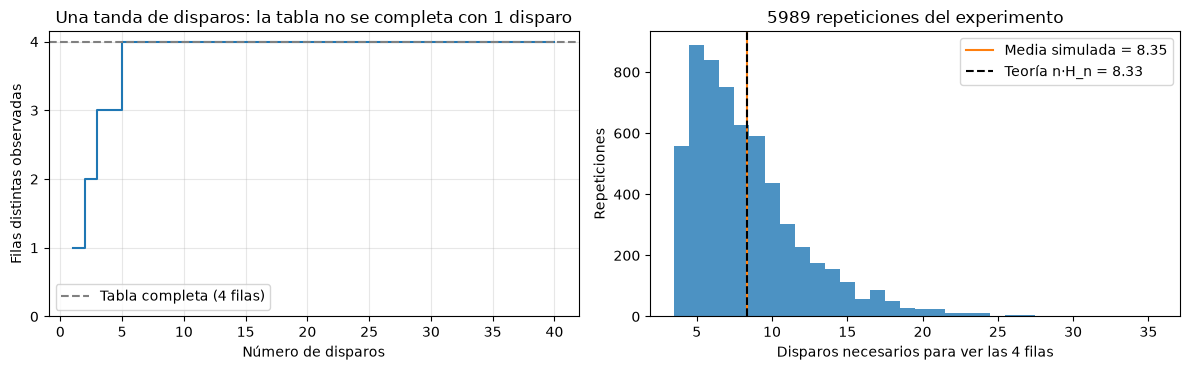
\includegraphics[width=\textwidth]{imagenes/bloque1/e1_3_experimento_1_disparo.png}
    \caption{Experimento de un solo disparo en el ejercicio 1.3 (XOR).
    Izquierda: filas distintas observadas en función del número de disparos en una tanda; la curva parte de una sola fila y necesita varios disparos para llegar a las cuatro.
    Derecha: histograma del número de disparos necesarios para observar las cuatro filas, repitiendo el experimento 5989 veces; la media simulada ($8{,}35$)
    coincide con la teórica $nH_n=25/3\approx 8{,}33$.}\label{fig:bloque1_e1_3_experimento}
\end{figure}

El histograma de la derecha de la Figura~\ref{fig:bloque1_e1_3_experimento} muestra que el mínimo número de disparos necesarios es 4 y que la distribución presenta una cola larga hacia la derecha
(en algunas repeticiones se necesitan más de 20 disparos, e incluso más de 30). Incluso con exactamente 4 disparos solo se obtiene la tabla completa con probabilidad
$4!/4^4=24/256\approx 9{,}4\%$, mientras que con un solo disparo esa probabilidad es exactamente 0. Los resultados son los mismos que con el AND del ejercicio 1.2, como cabe esperar:
el número de disparos necesarios depende solo de que las cuatro filas sean equiprobables, no de la función $f$ implementada.

\textbf{Resultado.} La simulación reproduce las cuatro cadenas previstas con probabilidad $\approx 1/4$ cada una y ninguna otra (Tabla~\ref{tab:bloque1_e1_3_super});
el test $\chi^2$ da un $p$-valor de $0{,}723$, compatible con la teoría al $5\%$. Cada disparo devuelve una sola fila $(a,f(a))$, por lo que un único disparo no da la tabla completa:
hacen falta en media $8{,}35$ disparos para observar las cuatro filas, en excelente acuerdo con el valor teórico $25/3\approx8{,}33$.

Obsérvese que esta $f$ vale 0 en dos entradas y 1 en las otras dos, es decir, es \emph{balanceada}, mientras que el AND del ejercicio 1.1 no lo es.
Esta distinción es la que aprovechará el algoritmo de Deutsch-Jozsa en el Bloque~3.

%--------------------------------------------------------------------
\subsection{Ejercicio 1.4. Oráculo de 3 bits con puertas multicontroladas}
La función vale 1 solo en tres entradas, por lo que basta una puerta multicontrolada por minitérmino ($x_2x_1x_0\in\{001,\,101,\,111\}$), todas con objetivo
$q_3\equiv y$ y controles en $q_0\equiv x_0$, $q_1\equiv x_1$, $q_2\equiv x_2$. Un control actúa sobre $|0\rangle$ (círculo blanco) cuando el bit correspondiente
del minitérmino es 0 (Tabla~\ref{tab:bloque1_e1_4_minterminos}).

\begin{table}[h]
    \centering
    \begin{tabular}{c|c|c}
    \hline
    Minitérmino $x_2x_1x_0$ & Controles sobre $|1\rangle$ & Controles sobre $|0\rangle$ \\
    \hline
    \texttt{001} & $q_0$ & $q_1,\,q_2$ \\
    \texttt{101} & $q_0,\,q_2$ & $q_1$ \\
    \texttt{111} & $q_0,\,q_1,\,q_2$ & ninguno \\
    \hline
    \end{tabular}
    \caption{Controles de cada puerta multicontrolada del oráculo del ejercicio 1.4.}\label{tab:bloque1_e1_4_minterminos}
\end{table}

Se utiliza \texttt{MCXGate(3, ctrl\_state=x)}, que equivale a rodear con puertas $X$ los controles que actúan sobre $|0\rangle$. En la
Figura~\ref{fig:bloque1_e1_4_oraculos} se muestran las dos versiones del oráculo; se comprueba que implementan el mismo operador.

\begin{figure}[htbp]
    \centering
    \begin{subfigure}{0.3\textwidth}
        \centering
        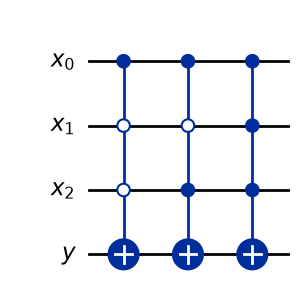
\includegraphics[width=\textwidth]{imagenes/bloque1/e1_4_oraculo3bits.png}
        \caption{Con \texttt{ctrl\_state}.}
    \end{subfigure}
    \hfill
    \begin{subfigure}{0.65\textwidth}
        \centering
        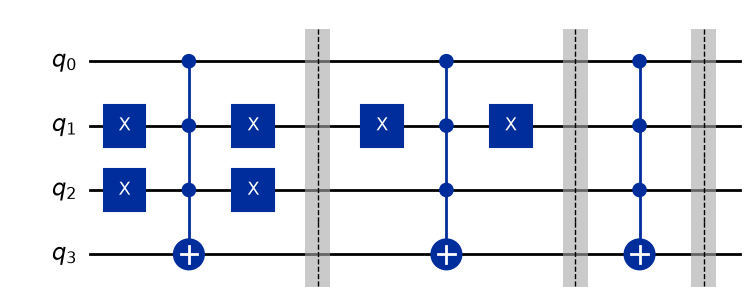
\includegraphics[width=\textwidth]{imagenes/bloque1/e1_4_oraculo3bit_impl.png}
        \caption{Con puertas $X$ explícitas.}
    \end{subfigure}
    \caption{Oráculo de 3 bits del ejercicio 1.4.}\label{fig:bloque1_e1_4_oraculos}
\end{figure}

Para comprobar el oráculo se prepara cada una de las ocho entradas con puertas $X$, se aplica $U_f$ y se miden los cuatro qubits (cadena \texttt{y x2 x1 x0}).
La Figura~\ref{fig:bloque1_e1_4_prueba} muestra, como ejemplo, el circuito de prueba para la entrada $x_2x_1x_0=101$, y la Tabla~\ref{tab:bloque1_e1_4} recoge el resultado para las ocho entradas.

\begin{figure}[h]
    \centering
    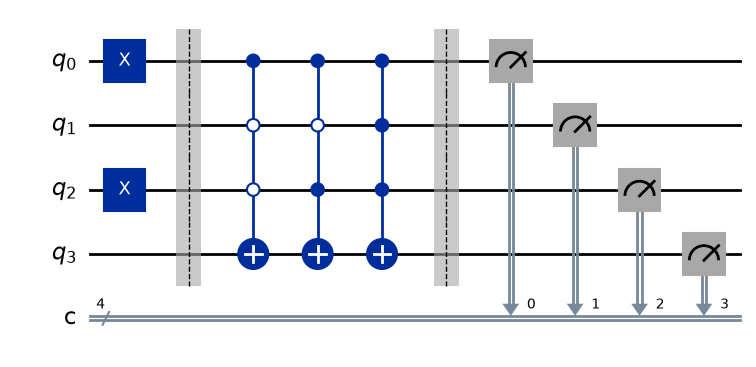
\includegraphics[width=0.6\textwidth]{imagenes/bloque1/e1_4_circuito_prueba.png}
    \caption{Circuito de prueba para la entrada $x_2x_1x_0=101$.}\label{fig:bloque1_e1_4_prueba}
\end{figure}

\begin{table}[htbp]
    \centering
\begin{tabular}{c|c|c|c|c}
\hline
$x_2x_1x_0$ & $f(x)$ teórica & $f(x)$ simulada & $x$ tras $U_f$ & Prob. \\
\hline
\texttt{000} & \texttt{0} & \texttt{0} & \texttt{000} & 1 \\
\texttt{001} & \texttt{1} & \texttt{1} & \texttt{001} & 1 \\
\texttt{010} & \texttt{0} & \texttt{0} & \texttt{010} & 1 \\
\texttt{011} & \texttt{0} & \texttt{0} & \texttt{011} & 1 \\
\texttt{100} & \texttt{0} & \texttt{0} & \texttt{100} & 1 \\
\texttt{101} & \texttt{1} & \texttt{1} & \texttt{101} & 1 \\
\texttt{110} & \texttt{0} & \texttt{0} & \texttt{110} & 1 \\
\texttt{111} & \texttt{1} & \texttt{1} & \texttt{111} & 1 \\
\hline
\end{tabular}
    \caption{Ejercicio 1.4: tabla de verdad simulada junto a la teórica.}\label{tab:bloque1_e1_4}
\end{table}

\textbf{Resultado.} Las ocho entradas producen $y=f(x)$ con probabilidad 1 y sin alterar $x$: la salida es 1 únicamente para $x_2x_1x_0=001,\,101,\,111$,
tal como indica la tabla del enunciado. Cada minitérmino activa una sola de las tres puertas, porque cada una solo se dispara con su propia entrada; por eso basta con componerlas
(se suman módulo 2 sobre $y$ sin solaparse). El operador coincide con el de la construcción con puertas $X$ explícitas y cumple $U_f^2=I$.

%--------------------------------------------------------------------
\subsection{Ejercicio 1.5. Oráculo de 4 bits de entrada y 4 de salida}
La tabla de la función se codifica en un diccionario de Python \texttt{\{`x3x2x1x0': `f3f2f1f0'\}} y el circuito se genera automáticamente recorriendo sus filas:
por cada fila y por cada bit $f_j=1$ se añade una \texttt{MCXGate(4)} con controles en $q_0\dots q_3$ (con \texttt{ctrl\_state} igual al propio $x$) y objetivo en $q_{4+j}$.
Las entradas están en $q_0\dots q_3$ y las salidas en $q_4\dots q_7$, siguiendo la cabecera de la tabla: $f_0\to q_4$ y $f_3\to q_7$.

\textbf{Predicción.} El número de puertas multicontroladas debe ser igual al número total de unos de la tabla, que es 32, y la cadena medida es \texttt{f3 f2 f1 f0 x3 x2 x1 x0}.
En el circuito generado (Figura~\ref{fig:bloque1_e1_5_oraculo}) se obtienen, en efecto, 32 puertas.

\begin{figure}[h]
    \centering
    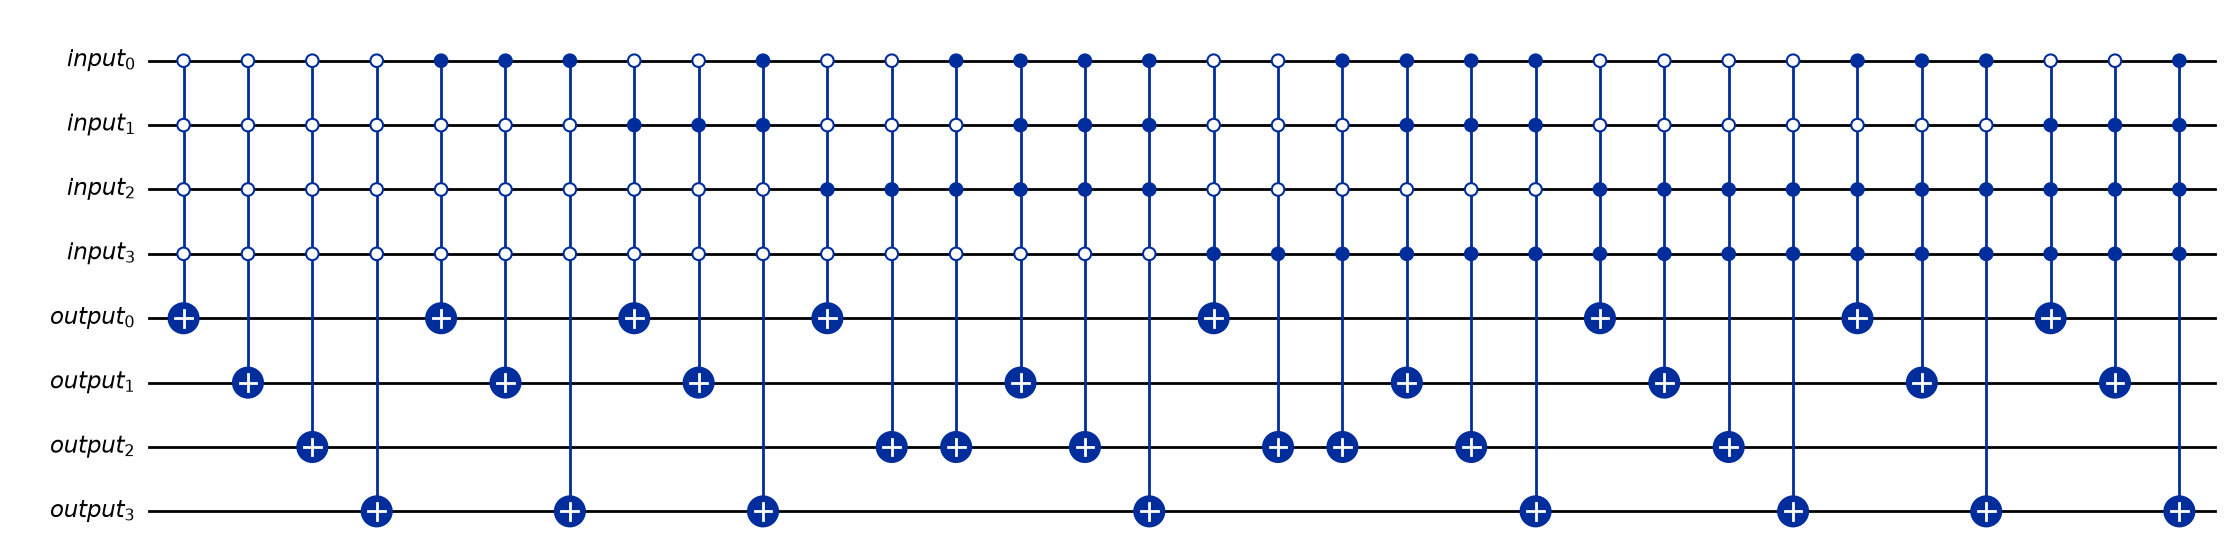
\includegraphics[width=\textwidth]{imagenes/bloque1/e1_5_oraculos4bits.png}
    \caption{Oráculo del ejercicio 1.5 (32 puertas multicontroladas).}\label{fig:bloque1_e1_5_oraculo}
\end{figure}

\begin{table}[htbp]
    \centering
{\small\setlength{\tabcolsep}{4pt}
\begin{tabular}{c|c|c|c||c|c|c|c}
\hline
$x_3x_2x_1x_0$ & teórica & simulada & Prob. & $x_3x_2x_1x_0$ & teórica & simulada & Prob. \\
\hline
\texttt{0000} & \texttt{1111} & \texttt{1111} & 1 & \texttt{1000} & \texttt{0101} & \texttt{0101} & 1 \\
\texttt{0001} & \texttt{1011} & \texttt{1011} & 1 & \texttt{1001} & \texttt{0100} & \texttt{0100} & 1 \\
\texttt{0010} & \texttt{0011} & \texttt{0011} & 1 & \texttt{1010} & \texttt{0000} & \texttt{0000} & 1 \\
\texttt{0011} & \texttt{1000} & \texttt{1000} & 1 & \texttt{1011} & \texttt{1110} & \texttt{1110} & 1 \\
\texttt{0100} & \texttt{0101} & \texttt{0101} & 1 & \texttt{1100} & \texttt{1111} & \texttt{1111} & 1 \\
\texttt{0101} & \texttt{0100} & \texttt{0100} & 1 & \texttt{1101} & \texttt{1011} & \texttt{1011} & 1 \\
\texttt{0110} & \texttt{0000} & \texttt{0000} & 1 & \texttt{1110} & \texttt{0011} & \texttt{0011} & 1 \\
\texttt{0111} & \texttt{1110} & \texttt{1110} & 1 & \texttt{1111} & \texttt{1000} & \texttt{1000} & 1 \\
\hline
\end{tabular}}
    \caption{Ejercicio 1.5: $f_3f_2f_1f_0$ teórica y simulada para las 16 entradas, con la probabilidad (frecuencia sobre 4096 disparos) con la que se obtiene
    cada resultado. En los 16 casos la entrada se mide intacta tras $U_f$.}\label{tab:bloque1_e1_5}
\end{table}

\textbf{Resultado.} Las 16 entradas dan la salida de la tabla con probabilidad 1 y las entradas quedan intactas (Tabla~\ref{tab:bloque1_e1_5}).
Esta función $f:\{0,1\}^4\to\{0,1\}^4$ no es inyectiva (hay salidas repetidas, como \texttt{0101} o \texttt{1111}), por lo que por sí sola no sería reversible. Sin embargo, el oráculo $U_f$
es siempre unitario e involutivo, gracias a que la entrada se conserva y la salida se suma módulo 2: su matriz es una permutación de la base computacional
de 8 qubits y cumple $U_f^2=I$, como se ha comprobado numéricamente.



%--------------------------------------------------------------------
\subsection{Ejercicio 1.6. Función lineal $f(x) = a\cdot x$}
Para $a=a_4a_3a_2a_1a_0=11010$ se tiene $f(x)=a\cdot x=x_4\oplus x_3\oplus x_1$. Una función lineal no necesita puertas multicontroladas:
basta un CNOT desde cada qubit $q_i\equiv x_i$ con $a_i=1$ hacia la ancilla $q_5\equiv y$. En este caso son tres CNOT, desde $q_4$, $q_3$ y $q_1$
(Figura~\ref{fig:bloque1_e1_6_oraculo}).

\begin{figure}[h]
    \centering
    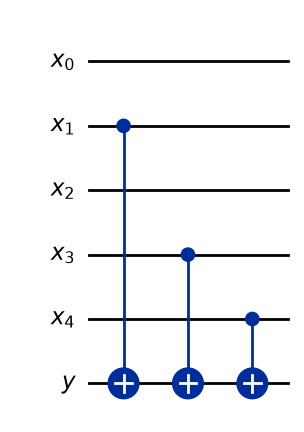
\includegraphics[width=0.3\textwidth]{imagenes/bloque1/e1_6_oraculosBV.png}
    \caption{Oráculo lineal $f(x)=x_4\oplus x_3\oplus x_1$.}\label{fig:bloque1_e1_6_oraculo}
\end{figure}

\textbf{Predicción.} $y=1$ exactamente en las entradas con un número impar de unos entre $x_4,x_3,x_1$ (16 de las 32), y la cadena medida es \texttt{y x4 x3 x2 x1 x0}.

\begin{table}[htbp]
    \centering
{\small\setlength{\tabcolsep}{4pt}
\begin{tabular}{c|c|c|c||c|c|c|c}
\hline
$x_4x_3x_2x_1x_0$ & teórica & simulada & Prob. & $x_4x_3x_2x_1x_0$ & teórica & simulada & Prob. \\
\hline
\texttt{00000} & \texttt{0} & \texttt{0} & 1 & \texttt{10000} & \texttt{1} & \texttt{1} & 1 \\
\texttt{00001} & \texttt{0} & \texttt{0} & 1 & \texttt{10001} & \texttt{1} & \texttt{1} & 1 \\
\texttt{00010} & \texttt{1} & \texttt{1} & 1 & \texttt{10010} & \texttt{0} & \texttt{0} & 1 \\
\texttt{00011} & \texttt{1} & \texttt{1} & 1 & \texttt{10011} & \texttt{0} & \texttt{0} & 1 \\
\texttt{00100} & \texttt{0} & \texttt{0} & 1 & \texttt{10100} & \texttt{1} & \texttt{1} & 1 \\
\texttt{00101} & \texttt{0} & \texttt{0} & 1 & \texttt{10101} & \texttt{1} & \texttt{1} & 1 \\
\texttt{00110} & \texttt{1} & \texttt{1} & 1 & \texttt{10110} & \texttt{0} & \texttt{0} & 1 \\
\texttt{00111} & \texttt{1} & \texttt{1} & 1 & \texttt{10111} & \texttt{0} & \texttt{0} & 1 \\
\texttt{01000} & \texttt{1} & \texttt{1} & 1 & \texttt{11000} & \texttt{0} & \texttt{0} & 1 \\
\texttt{01001} & \texttt{1} & \texttt{1} & 1 & \texttt{11001} & \texttt{0} & \texttt{0} & 1 \\
\texttt{01010} & \texttt{0} & \texttt{0} & 1 & \texttt{11010} & \texttt{1} & \texttt{1} & 1 \\
\texttt{01011} & \texttt{0} & \texttt{0} & 1 & \texttt{11011} & \texttt{1} & \texttt{1} & 1 \\
\texttt{01100} & \texttt{1} & \texttt{1} & 1 & \texttt{11100} & \texttt{0} & \texttt{0} & 1 \\
\texttt{01101} & \texttt{1} & \texttt{1} & 1 & \texttt{11101} & \texttt{0} & \texttt{0} & 1 \\
\texttt{01110} & \texttt{0} & \texttt{0} & 1 & \texttt{11110} & \texttt{1} & \texttt{1} & 1 \\
\texttt{01111} & \texttt{0} & \texttt{0} & 1 & \texttt{11111} & \texttt{1} & \texttt{1} & 1 \\
\hline
\end{tabular}}
    \caption{Ejercicio 1.6: $f(x)=x_4\oplus x_3\oplus x_1$ para las 32 entradas, con el valor teórico, el simulado y la probabilidad con la que se obtiene
    (frecuencia sobre 4096 disparos). En los 32 casos la entrada se mide intacta tras $U_f$.}\label{tab:bloque1_e1_6}
\end{table}

\textbf{Resultado.} Las 32 entradas coinciden con $f(x)=x_4\oplus x_3\oplus x_1$ (paridad de los bits de $x$ en las posiciones donde $a$ vale 1) con probabilidad 1,
y $x$ no se modifica (Tabla~\ref{tab:bloque1_e1_6}). El oráculo usa solo 3 CNOT, frente a las 16 puertas multicontroladas que requeriría la construcción por minitérminos
para esta función (16 entradas con $f=1$). Este mismo oráculo se reutiliza en el algoritmo de Bernstein-Vazirani (ejercicio 3.3), donde la cadena oculta $a$ se recupera con una única consulta.